% Created by tikzDevice version 0.12.6 on 2024-08-01 12:50:13
% !TEX encoding = UTF-8 Unicode
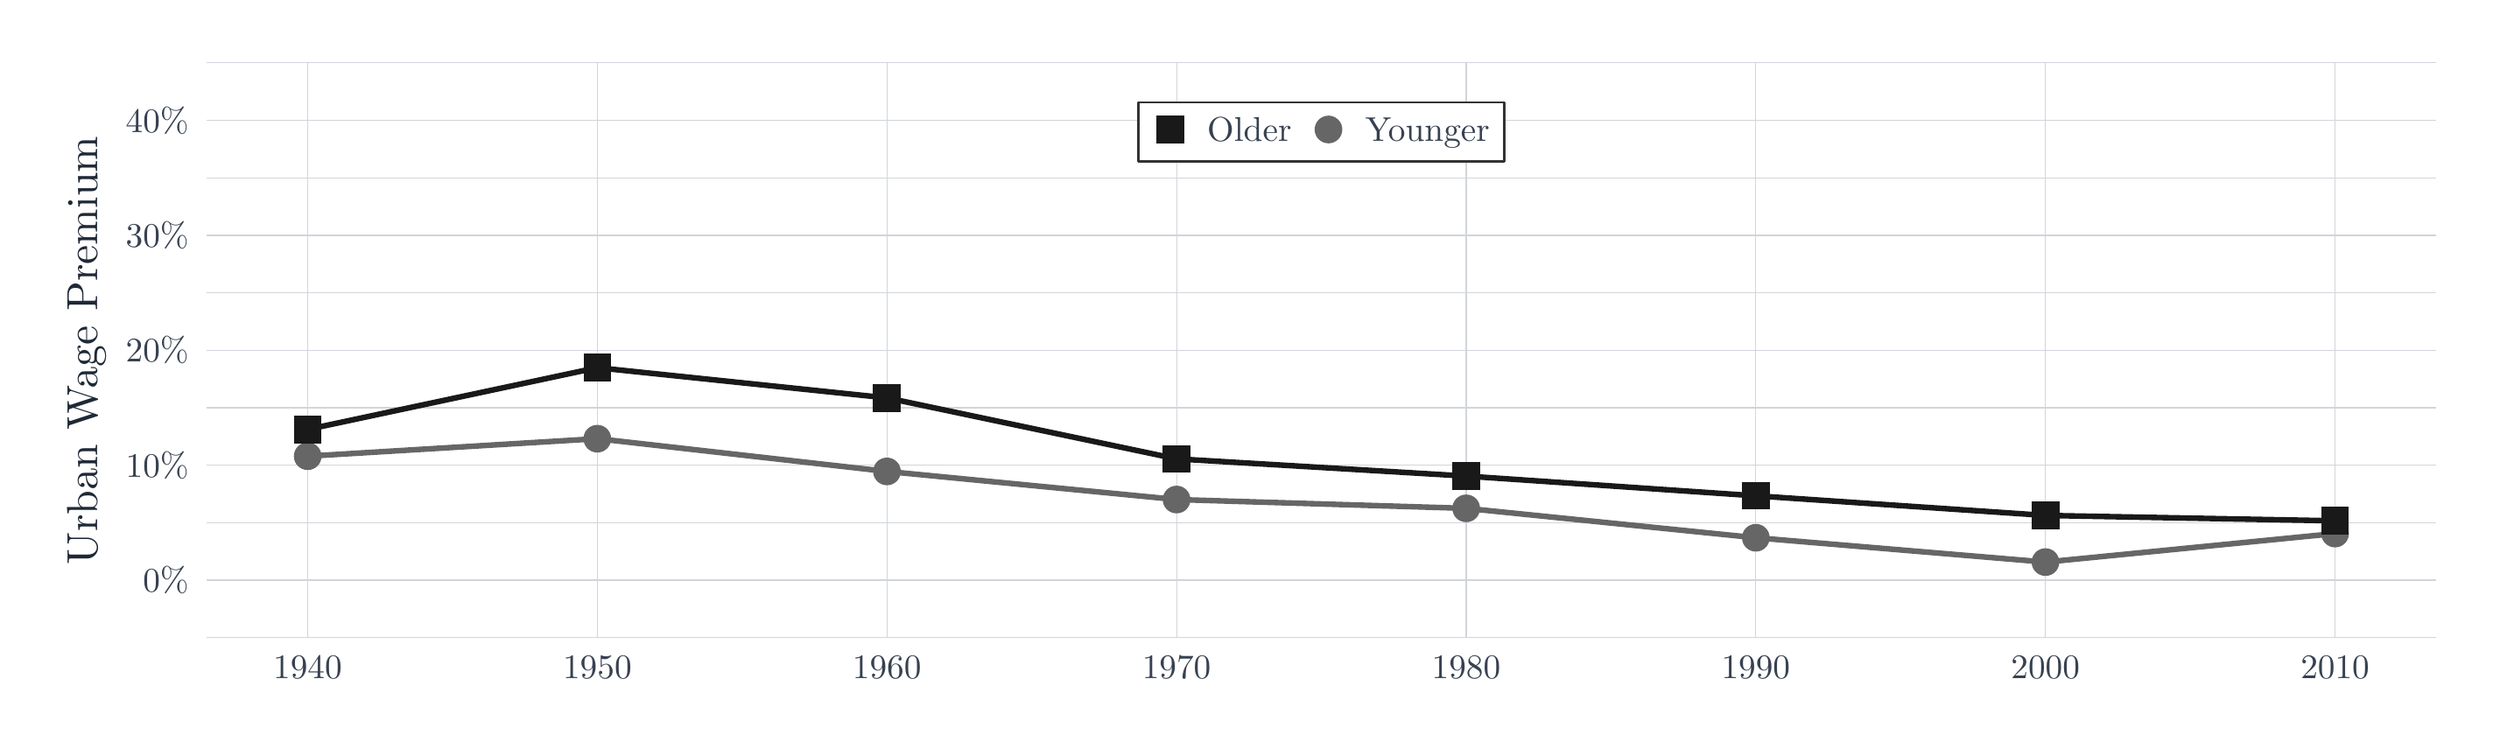
\begin{tikzpicture}[x=1pt,y=1pt]
\definecolor{fillColor}{RGB}{255,255,255}
\path[use as bounding box,fill=fillColor] (0,0) rectangle (1011.78,289.08);
\begin{scope}
\path[clip] (  0.00,  0.00) rectangle (1011.78,289.08);
\definecolor{drawColor}{RGB}{255,255,255}

\path[draw=drawColor,line width= 0.8pt,line join=round,line cap=round,fill=fillColor] (  0.00,  0.00) rectangle (1011.78,289.08);
\end{scope}
\begin{scope}
\path[clip] ( 75.16, 35.76) rectangle (995.78,273.08);
\definecolor{drawColor}{RGB}{255,255,255}
\definecolor{fillColor}{RGB}{255,255,255}

\path[draw=drawColor,line width= 0.8pt,line join=round,line cap=round,fill=fillColor] ( 75.16, 35.76) rectangle (995.78,273.08);
\definecolor{drawColor}{RGB}{209,213,219}

\path[draw=drawColor,line width= 0.4pt,line join=round] ( 75.16, 35.76) --
	(995.78, 35.76);

\path[draw=drawColor,line width= 0.4pt,line join=round] ( 75.16, 83.22) --
	(995.78, 83.22);

\path[draw=drawColor,line width= 0.4pt,line join=round] ( 75.16,130.69) --
	(995.78,130.69);

\path[draw=drawColor,line width= 0.4pt,line join=round] ( 75.16,178.15) --
	(995.78,178.15);

\path[draw=drawColor,line width= 0.4pt,line join=round] ( 75.16,225.62) --
	(995.78,225.62);

\path[draw=drawColor,line width= 0.4pt,line join=round] ( 75.16,273.08) --
	(995.78,273.08);

\path[draw=drawColor,line width= 0.4pt,line join=round] ( 75.16, 59.49) --
	(995.78, 59.49);

\path[draw=drawColor,line width= 0.4pt,line join=round] ( 75.16,106.95) --
	(995.78,106.95);

\path[draw=drawColor,line width= 0.4pt,line join=round] ( 75.16,154.42) --
	(995.78,154.42);

\path[draw=drawColor,line width= 0.4pt,line join=round] ( 75.16,201.88) --
	(995.78,201.88);

\path[draw=drawColor,line width= 0.4pt,line join=round] ( 75.16,249.35) --
	(995.78,249.35);

\path[draw=drawColor,line width= 0.4pt,line join=round] (117.01, 35.76) --
	(117.01,273.08);

\path[draw=drawColor,line width= 0.4pt,line join=round] (236.57, 35.76) --
	(236.57,273.08);

\path[draw=drawColor,line width= 0.4pt,line join=round] (356.13, 35.76) --
	(356.13,273.08);

\path[draw=drawColor,line width= 0.4pt,line join=round] (475.69, 35.76) --
	(475.69,273.08);

\path[draw=drawColor,line width= 0.4pt,line join=round] (595.25, 35.76) --
	(595.25,273.08);

\path[draw=drawColor,line width= 0.4pt,line join=round] (714.81, 35.76) --
	(714.81,273.08);

\path[draw=drawColor,line width= 0.4pt,line join=round] (834.37, 35.76) --
	(834.37,273.08);

\path[draw=drawColor,line width= 0.4pt,line join=round] (953.93, 35.76) --
	(953.93,273.08);
\definecolor{drawColor}{gray}{0.10}

\path[draw=drawColor,line width= 2.3pt,line join=round] (117.01,121.74) --
	(236.57,147.23) --
	(356.13,134.76) --
	(475.69,109.58) --
	(595.25,102.47) --
	(714.81, 94.32) --
	(834.37, 86.22) --
	(953.93, 83.99);
\definecolor{drawColor}{gray}{0.40}

\path[draw=drawColor,line width= 2.3pt,line join=round] (117.01,110.68) --
	(236.57,117.91) --
	(356.13,104.39) --
	(475.69, 92.78) --
	(595.25, 89.14) --
	(714.81, 77.00) --
	(834.37, 66.95) --
	(953.93, 78.73);
\definecolor{fillColor}{gray}{0.40}

\path[fill=fillColor] (117.01,110.68) circle (  5.71);
\definecolor{fillColor}{gray}{0.10}

\path[fill=fillColor] (111.30,116.03) --
	(122.72,116.03) --
	(122.72,127.45) --
	(111.30,127.45) --
	cycle;
\definecolor{fillColor}{gray}{0.40}

\path[fill=fillColor] (236.57,117.91) circle (  5.71);
\definecolor{fillColor}{gray}{0.10}

\path[fill=fillColor] (230.86,141.52) --
	(242.28,141.52) --
	(242.28,152.94) --
	(230.86,152.94) --
	cycle;
\definecolor{fillColor}{gray}{0.40}

\path[fill=fillColor] (356.13,104.39) circle (  5.71);
\definecolor{fillColor}{gray}{0.10}

\path[fill=fillColor] (350.42,129.05) --
	(361.84,129.05) --
	(361.84,140.47) --
	(350.42,140.47) --
	cycle;
\definecolor{fillColor}{gray}{0.40}

\path[fill=fillColor] (475.69, 92.78) circle (  5.71);
\definecolor{fillColor}{gray}{0.10}

\path[fill=fillColor] (469.98,103.87) --
	(481.40,103.87) --
	(481.40,115.29) --
	(469.98,115.29) --
	cycle;
\definecolor{fillColor}{gray}{0.40}

\path[fill=fillColor] (595.25, 89.14) circle (  5.71);
\definecolor{fillColor}{gray}{0.10}

\path[fill=fillColor] (589.54, 96.76) --
	(600.96, 96.76) --
	(600.96,108.18) --
	(589.54,108.18) --
	cycle;
\definecolor{fillColor}{gray}{0.40}

\path[fill=fillColor] (714.81, 77.00) circle (  5.71);
\definecolor{fillColor}{gray}{0.10}

\path[fill=fillColor] (709.10, 88.61) --
	(720.52, 88.61) --
	(720.52,100.03) --
	(709.10,100.03) --
	cycle;
\definecolor{fillColor}{gray}{0.40}

\path[fill=fillColor] (834.37, 66.95) circle (  5.71);
\definecolor{fillColor}{gray}{0.10}

\path[fill=fillColor] (828.66, 80.51) --
	(840.08, 80.51) --
	(840.08, 91.93) --
	(828.66, 91.93) --
	cycle;
\definecolor{fillColor}{gray}{0.40}

\path[fill=fillColor] (953.93, 78.73) circle (  5.71);
\definecolor{fillColor}{gray}{0.10}

\path[fill=fillColor] (948.22, 78.28) --
	(959.64, 78.28) --
	(959.64, 89.70) --
	(948.22, 89.70) --
	cycle;
\end{scope}
\begin{scope}
\path[clip] (  0.00,  0.00) rectangle (1011.78,289.08);
\definecolor{drawColor}{RGB}{55,65,81}

\node[text=drawColor,anchor=base east,inner sep=0pt, outer sep=0pt, scale=  1.42] at ( 67.96, 54.59) {0\%};

\node[text=drawColor,anchor=base east,inner sep=0pt, outer sep=0pt, scale=  1.42] at ( 67.96,102.06) {10\%};

\node[text=drawColor,anchor=base east,inner sep=0pt, outer sep=0pt, scale=  1.42] at ( 67.96,149.52) {20\%};

\node[text=drawColor,anchor=base east,inner sep=0pt, outer sep=0pt, scale=  1.42] at ( 67.96,196.99) {30\%};

\node[text=drawColor,anchor=base east,inner sep=0pt, outer sep=0pt, scale=  1.42] at ( 67.96,244.45) {40\%};
\end{scope}
\begin{scope}
\path[clip] (  0.00,  0.00) rectangle (1011.78,289.08);
\definecolor{drawColor}{RGB}{55,65,81}

\node[text=drawColor,anchor=base,inner sep=0pt, outer sep=0pt, scale=  1.42] at (117.01, 18.76) {1940};

\node[text=drawColor,anchor=base,inner sep=0pt, outer sep=0pt, scale=  1.42] at (236.57, 18.76) {1950};

\node[text=drawColor,anchor=base,inner sep=0pt, outer sep=0pt, scale=  1.42] at (356.13, 18.76) {1960};

\node[text=drawColor,anchor=base,inner sep=0pt, outer sep=0pt, scale=  1.42] at (475.69, 18.76) {1970};

\node[text=drawColor,anchor=base,inner sep=0pt, outer sep=0pt, scale=  1.42] at (595.25, 18.76) {1980};

\node[text=drawColor,anchor=base,inner sep=0pt, outer sep=0pt, scale=  1.42] at (714.81, 18.76) {1990};

\node[text=drawColor,anchor=base,inner sep=0pt, outer sep=0pt, scale=  1.42] at (834.37, 18.76) {2000};

\node[text=drawColor,anchor=base,inner sep=0pt, outer sep=0pt, scale=  1.42] at (953.93, 18.76) {2010};
\end{scope}
\begin{scope}
\path[clip] (  0.00,  0.00) rectangle (1011.78,289.08);
\definecolor{drawColor}{RGB}{31,41,55}

\node[text=drawColor,rotate= 90.00,anchor=base,inner sep=0pt, outer sep=0pt, scale=  1.80] at ( 30.15,154.42) {Urban Wage Premium};
\end{scope}
\begin{scope}
\path[clip] (  0.00,  0.00) rectangle (1011.78,289.08);
\definecolor{drawColor}{gray}{0.20}
\definecolor{fillColor}{RGB}{255,255,255}

\path[draw=drawColor,line width= 0.8pt,line join=round,line cap=round,fill=fillColor] (459.93,232.37) rectangle (611.01,256.83);
\end{scope}
\begin{scope}
\path[clip] (  0.00,  0.00) rectangle (1011.78,289.08);
\definecolor{drawColor}{RGB}{255,255,255}
\definecolor{fillColor}{RGB}{255,255,255}

\path[draw=drawColor,line width= 0.8pt,line join=round,line cap=round,fill=fillColor] (465.93,238.37) rectangle (480.39,252.83);
\end{scope}
\begin{scope}
\path[clip] (  0.00,  0.00) rectangle (1011.78,289.08);
\definecolor{fillColor}{gray}{0.10}

\path[fill=fillColor] (467.45,239.89) --
	(478.87,239.89) --
	(478.87,251.31) --
	(467.45,251.31) --
	cycle;
\end{scope}
\begin{scope}
\path[clip] (  0.00,  0.00) rectangle (1011.78,289.08);
\definecolor{drawColor}{RGB}{255,255,255}
\definecolor{fillColor}{RGB}{255,255,255}

\path[draw=drawColor,line width= 0.8pt,line join=round,line cap=round,fill=fillColor] (531.18,238.37) rectangle (545.63,252.83);
\end{scope}
\begin{scope}
\path[clip] (  0.00,  0.00) rectangle (1011.78,289.08);
\definecolor{fillColor}{gray}{0.40}

\path[fill=fillColor] (538.40,245.60) circle (  5.71);
\end{scope}
\begin{scope}
\path[clip] (  0.00,  0.00) rectangle (1011.78,289.08);
\definecolor{drawColor}{RGB}{55,65,81}

\node[text=drawColor,anchor=base west,inner sep=0pt, outer sep=0pt, scale=  1.42] at (488.39,240.70) {Older};
\end{scope}
\begin{scope}
\path[clip] (  0.00,  0.00) rectangle (1011.78,289.08);
\definecolor{drawColor}{RGB}{55,65,81}

\node[text=drawColor,anchor=base west,inner sep=0pt, outer sep=0pt, scale=  1.42] at (553.63,240.70) {Younger};
\end{scope}
\end{tikzpicture}
